\begin{figure}
    \centering
    \begin{subfigure}{0.45\textwidth}
        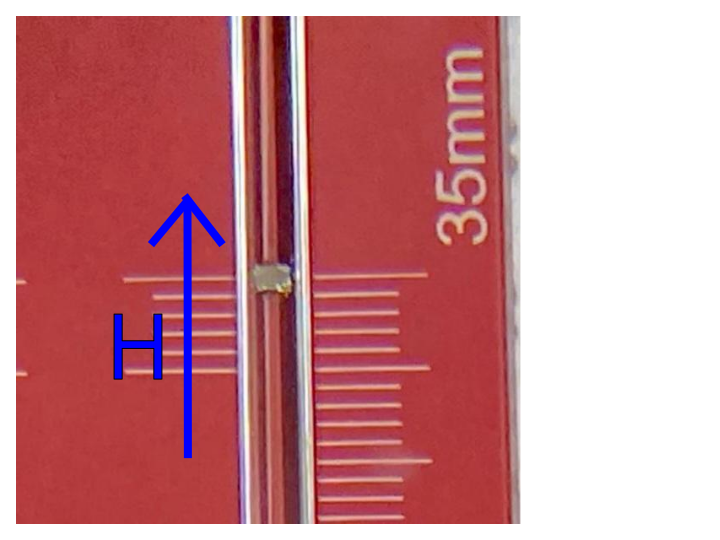
\includegraphics[width=1.4\linewidth]{pdf_files/sample_a_arrow.pdf}
        \caption{First position of sample, with the magnetic field along the a-axis.}
        \label{fig:original-sample}
    \end{subfigure} \hfill
    \begin{subfigure}{0.45\textwidth}
        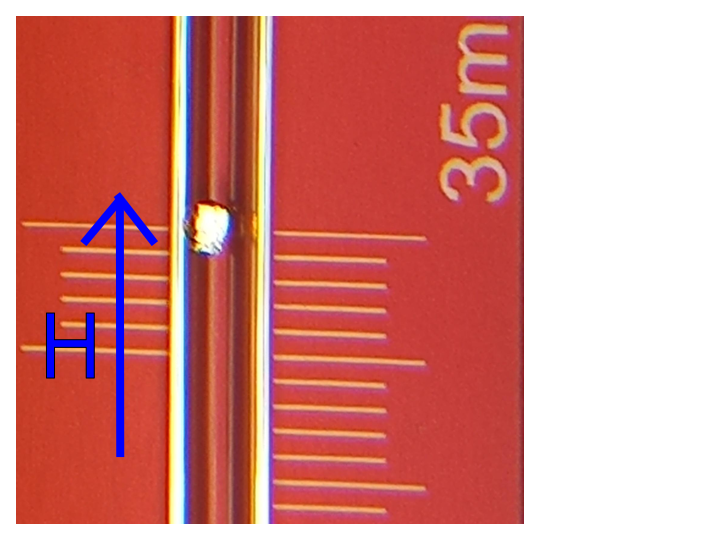
\includegraphics[width=1.4\linewidth]{pdf_files/sample_b_arrow.pdf}
        \caption{Second position of sample, with the magnetic field along the b-axis.}
        \label{fig:rotated-sample}
    \end{subfigure}
    \begin{subfigure}{0.45\textwidth}
        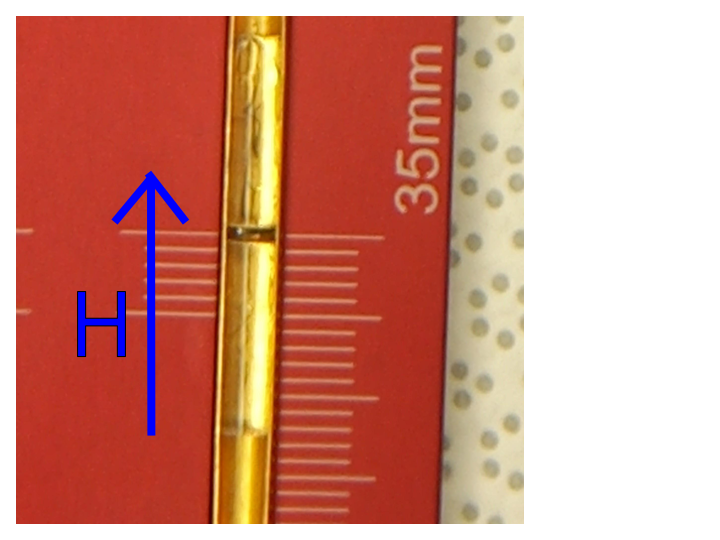
\includegraphics[width=1.4\linewidth]{pdf_files/sample_c_arrow.pdf}
        \caption{Third position of sample, with the magnetic field along the c-axis.}
        \label{fig:sample-pos-c}
    \end{subfigure}
    \caption{Sample mounted on holder before each M vs. T experiment. During each experiment, the magnetic field was going from the bottom to the top of the image, as shown by the blue arrows.}
    \label{fig:both-samples}
\end{figure}